% !TeX encoding = UTF-8
% !TeX program = pdfLaTeX
% !TeX spellcheck = en_US

\documentclass{beamer}

\usepackage[T1]{fontenc}
\usepackage[utf8]{inputenc}
\usepackage[english]{babel}
\usepackage{lmodern}
\usepackage{microtype}
\usepackage{beamerthemeshadow}
\usepackage{beamercolor}


\setbeamercolor*{palette primary} {use=structure,fg=white,bg=structure.fg}

\setbeamercolor*{palette secondary} {use=structure,fg=white,bg=structure.fg!75!black}
\setbeamercolor*{palette tertiary} {use=structure,fg=white,bg=structure.fg!50!black}
\setbeamercolor*{palette quaternary}{fg=white,bg=black}
\setbeamercolor*{sidebar}{use=structure ,bg=structure.fg}
\setbeamercolor*{palette sidebar primary} {use=structure ,fg=structure.fg!10}
\setbeamercolor*{palette sidebar secondary}{fg=white}
\setbeamercolor*{palette sidebar tertiary}{use=structure ,fg=structure.fg!50}
\setbeamercolor*{palette sidebar quaternary}{fg=white}
\setbeamercolor*{titlelike}{parent=palette primary} 
\setbeamercolor*{separation line}{}
\setbeamercolor*{fine separation line}{}

\frenchspacing

\graphicspath{{./img/}}

\title{
  \textsl{Pathrate} on mobile environments\texorpdfstring{\\}{--}
  An implementation on Android
}
\author{
  Antonio Macrì\texorpdfstring{ $\cdot$}{,}
  Francesco Racciatti\texorpdfstring{ $\cdot$}{,}
  Silvia Volpe
}
\date{\today}


\begin{document}

\frame{
  \titlepage
}

\frame{\frametitle{\contentsname}
  \tableofcontents
}


\section{How does \protect\textsl{pathrate} work}
\frame{
  \sectionpage
}

\subsection{Packet-pair technique}

\frame{\frametitle{Packet-pair technique}
  Two consecutive \emph{probing packets} leave the sender \emph{back-to-back}
  and arrive at the receiver with a \emph{dispersion} (spacing) that is
  determined by the \emph{narrow link} in the path.
  % Dispersion: time interval between the complete transmission (up to the last
  % bit) of two packets.

  \bigskip
  \begin{columns}
  \begin{column}{0.5\columnwidth}
  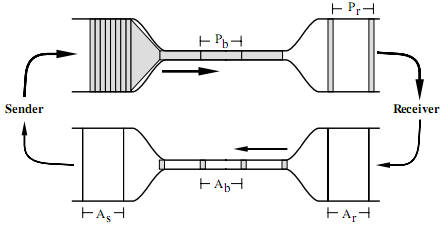
\includegraphics[width=\columnwidth]{self-clocking}
  \end{column}
  \begin{column}{0.2\columnwidth}
  $b = L/\delta$
  \end{column}
  \end{columns}
  \pause

  \bigskip
  Without any cross-traffic, measuring the dispersions and knowing the size of
  the packets, we can calculate the capacity of the narrow link (i.\,e. the
  capacity of the path) as $b = L/\delta$.
}

\subsection{Capacity modes}

\frame{\frametitle{Capacity modes}
  One problem arises because the distribution of the capacities is multimodal
  and the path capacity is likely to be the global mode only when the path is
  lightly loaded, but often it is \emph{not} the global mode.
  \pause

  \bigskip
  Capacity modes:
  \begin{itemize}
  \item \emph{Capacity Mode} (CM): the mode we are looking for
        % CM is formed by packet pairs that did not get queued behind cross
        % traffic packets in the path.
  \item \emph{Sub-Capacity Dispersion Range} (SCDR): due to cross-traffic
        packets that interfere with packet pairs increasing their dispersion
        ($<$ CM)
        % For example, when one cross traffic packet of the same size as the
        % probing packets interferes between packet pairs, the measured
        % capacity is half the actual capacity of the link.
        % Typically, in the Internet cross-traffic packet size is distributed
        % around three or four common values, and this explains the local
        % modes in the SCDR (rather than a uniform distribution).
        % Alex docet: attualmente la quasi totalità dei pacchetti che circolano in rete
        % hanno dimensione pari all'MTU di Ethernet
  \item \emph{Post-Narrow Capacity Modes} (PNCMs): when the probing packets
        get closer because the first packet encounters (in a post-narrow link)
        a greater delay than the second ($>$ CM)
        % Local modes in this portion of the histogram are created when the
        % first probing packet is delayed long enough for the packet pair to
        % be serviced back-to-back in that link (and all subsequent links have
        % higher capacities).
  \end{itemize}
}

\frame{\frametitle{Capacity modes (cont.)}
  \begin{center}
  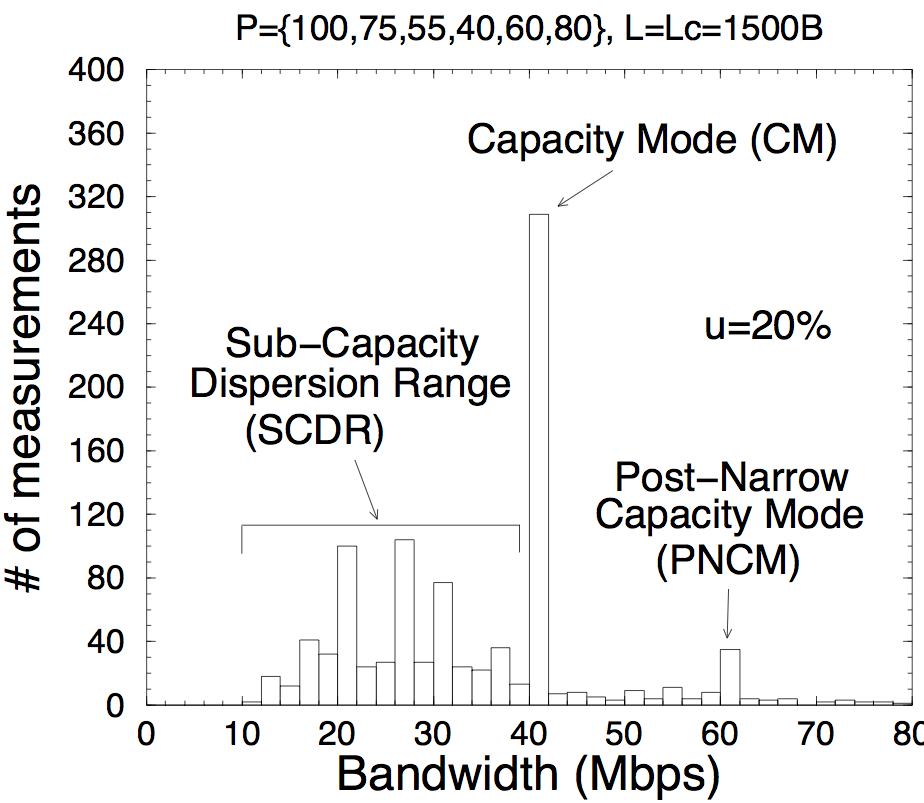
\includegraphics[width=0.48\columnwidth]{capacity-modes-u20}\quad
  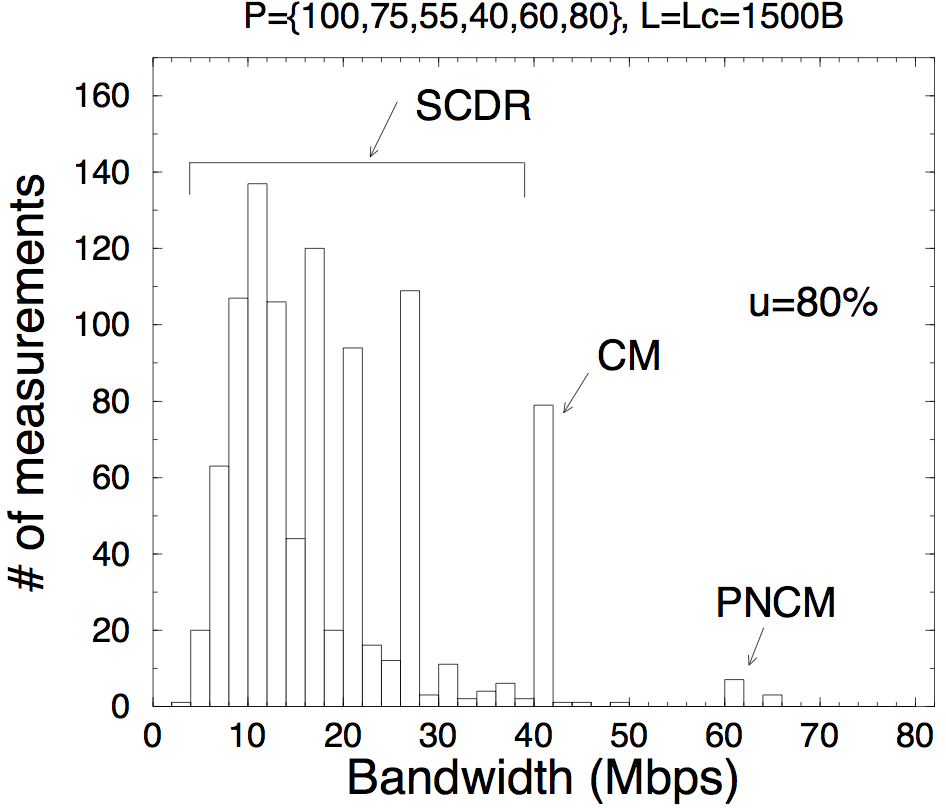
\includegraphics[width=0.48\columnwidth]{capacity-modes-u80}
  \end{center}
}

\frame{\frametitle{Capacity modes (cont.)}
  The path capacity cannot be estimated, in the general case, by statistical
  techniques that extract the most common bandwidth value or range, or from the
  maximum (or minimum) bandwidth measurement.
  \pause

  \medskip
  \begin{alertblock}{Capacity Mode}
  CM must be distinguished from SCDR and PNCM modes.
  \end{alertblock}

  \medskip
% TODO: eg a inizio frase non credo di sia mai visto nella storia
  e.g. in heavily congested paths, SCDR is prevalent and CM may not even appear as a
  local mode if almost every packet pair is affected by cross traffic. Even PNCM
  are less likely to appear.
}

\subsection{Choosing operative parameters}

\frame{\frametitle{Choosing operative parameters}
  So we must be able to recognize wrong estimations:
  \begin{itemize}
  \item underestimations due to cross-traffic (SCDR zone)
  \item overestimations due to non-empty buffers in some post-narrow node
        (PNCMs)
  \end{itemize} \pause

  \bigskip
  Workarounds:
  \begin{itemize}
  \item varying probing packet size among different packet pairs, so that the
        SCDR modes become wider and weaker, making the CM mode relatively
        stronger
  \item using probing packets as large as possible to reduce creation of PNCMs
        but not too large to determine predominance of SCDR
        % In pathrate, the minimum probing size is set to 550 bytes.
  \end{itemize}
}

\frame{\frametitle{Choosing operative parameters (cont.)}
  Note that the two packets of a pair \emph{must} have the same size, otherwise
  they encounter different transmission delays and can produce a dispersion
  also dependent on the size of the first packet.
  % Suppose that at link $i-1$ the two packets are traveling back-to-back and
  % that the transmission of the first packet on link $i$ is completed before
  % reception of the last bit of the second packet from link $i$. Varying the
  % size of the first packets causes the dispersion to change too.
  \pause

  \bigskip
  Using larger packet size (i.\,e. MTU) leads to wider dispersion that:
  \begin{itemize}
% TODO: “because packets should not be fragmented” che significa?s
  \item is easier to measure because packets should not be fragmented
  \item is less sensitive to the timestamping resolution at the receiver
  \item is more robust to queuing delay noise
  \item reduces the formation of PNCM
        % Because, if probing packet size is small compared to cross traffic
        % packets, it is sufficient a smaller amount of interfering cross
        % traffic to make packet pair depart from a post-narrow link
        % back-to-back.
  \setbeamercolor{item}{fg=red}
  \item is more subject to interfering cross traffic, an thus increases the
        predominance of SCDR
        % Because it is less likely for cross traffic packets to interfere
        % between small probing packets.
  \end{itemize}
}

\subsection{Packet pairs vs packet trains}

\frame{\frametitle{Packet trains}
  Generalization: send $N>2$ back-to-back packets of the same size $L$ and
  measure the total dispersion from the last bit of the first packet to the last
  bit of the last packet

  \bigskip
  A bandwidth measurement is calculated as follows:
  \[b(N) = \frac{(N-1)L}{\Delta(N)}\]
  \pause

  \bigskip
  Without cross traffic in the path, all measurements will be equal to the
  capacity, regardless of the value of $N$.
}

\frame{\frametitle{Packet trains (cont.)}
  But as the train length $N$ increases, more cross traffic packets can
  interfere with the packet train resulting in bandwidth measurements that are
  less than the path capacity.

  \bigskip
  As a consequence, the CM and PNCMs become weaker, until they disappear, and
  the SCDR prevails
  % This implies that the optimal train length for generating a strong capacity
  % mode is $N=2$, i.\,e. to use packet pairs.

  \bigskip
  When the train length $N$ is sufficiently large, bandwidth measurements are
  (almost always) less than the path capacity, and tend toward a single value
  leading to a unimodal distribution that becomes independent of~$N$

  % One should use trains when the narrow link is multichanneled: in a
  % $p$-channel link, should be $N=p+1$.
  % We actually ignore possible multichanneled links (just as in the original
  % paper).
}

\frame{\frametitle{Average Dispersion Rate}
  The resulting mode is referred to as \emph{Average Dispersion Rate} (ADR)

  \bigskip
  The ADR is a bandwidth metric that is not directly related to the (end-to-end)
  available bandwidth of the path, which depends on the utilization and capacity
  of only the tight link. Instead, the ADR is determined by the capacity and
  available bandwidth of \emph{each} link in the path
  % Dispersion of long packet trains is not related to the available bandwidth of
  % the path (as earlier works assumed): the mean of the packet train dispersion
  % distribution corresponds to the \emph{Average Dispersion Rate}, that depends
  % in general on the capacity and utilization of all links in the path as well as
  % on the routing of cross traffic relative to the measured path.
  \pause

  \medskip
  \begin{block}{ADR}
  The ADR is a lower bound of the capacity and an upper bound of the available
  bandwidth of the path.
  \end{block}
  % ADR is calculated as the mean packet train dispersion (for $N$ sufficiently
  % large).
}

\frame{\frametitle{Capacity estimation methodology}
  Principles:
  \begin{enumerate}
  \item use packet pairs, i.\,e. $N=2$
  \item variable-sized packets to make the SCDR modes wider
  \item prefer larger packets to make the PNCM weaker
  \item measure the ADR with long packet trains
  \end{enumerate}
  
  \bigskip
  Three execution phases:
  \begin{enumerate}
  \item Preliminary measurements and (possibly) “quick estimate”
        % In this phase, pathrate sends about 60 packet trains of at most
        % 10 packets length.
        % One goal is to calculate the bin width $\omega$ (they say as 10\% of
        % the interquartile range of the preliminary measurements). The final
        % capacity estimate will be a range of width $\omega$.
        % If the Coefficient Of Variation (COF) is less than 5\% (which happens
        % when the network is quite lightly loaded), the preliminary measurements
        % terminate with a “quick estimate”: is produced a “final capacity
        % estimate” as the average of the preliminary measurements (after
        % removing the 10\% smallest and largest values).
  \item Phase I: packet pair probing
        % A huge number (1000) of packet pairs is sent, with variable probing
        % packet sizes ($550 \div 1500$).
        % Using statistical procedures, pathrate identifies the local modes.
  \item Phase II: ADR estimation and Capacity Mode selection
        %
  \end{enumerate}
}


\section{Why \protect\textsl{pathrate} doesn't work in mobile environments} 
\frame{
  \sectionpage
}

\subsection{Problems in mobile environments}

\frame{\frametitle{Problems in mobile environments}
  Main problems of mobile environments are:
  \begin{itemize}
  \item CSMA/CA overhead reduces path capacity
  \item nodes in the same WLAN may compete to obtain access to the shared medium
  \item high BER
  \item energy saving policies
  \end{itemize}
}

\frame{\frametitle{Competing nodes \& BER}
  
  In a wireless environment there're many factors which increase measurement's uncertainty:
  %
  \begin{itemize}
  \item high amount of nodes which compete, i.e. high number of collisions and ritransmissions
  \item high BER, i.e. high number of ritrasmissions due to packet corruption
  \end{itemize}  
}

\frame{\frametitle{Energy saving policies}
  With the goal of energy saving, a node could:
% TODO: “with the goal of energy saving” mi suona male, sembra che manchi
%       qualcosa dopo “saving”. Secongo me ci sta più “energy efficiency” o
%       qualche altra espressione
  \begin{itemize}
  \item slow down NIC's rate
  \item adjust CPU frequency based on battery level
  \setbeamercolor{item}{fg=red}
  \item activate \emph{Interrupt Coalescence} (IC)
  \end{itemize}
}


\subsection{Interrupt Coelescence}

\frame{\frametitle{Interrupt Coelescence}
  It's a mechanism used to avoid flooding the OS with too many interrupts.
  Typically used in Gigabit Ethernet adapters, more recently is widely enabled
  in energy-constrained devices.

  \bigskip
  In a NAPI-compliant driver, when a packet arrives and the interface
  signals the event, the interrupt handler \emph{does not} process the packet.
  Instead it disables receive interrupts and tells the kernel to start
  \emph{polling} the interface.
  
 }
 
 \frame{\frametitle{Interrupt Coelescence (cont.)}

  Meanwile, the NAPI-capable interface stores received packets directly into the
  RAM via DMA 
  %(\emph{in-memory DMA ring}), 
  taking a substantial amount of load
  off the processor.

  \bigskip
  When the polling timer expires
  %(i.\,e.~when a certain time interval has elapsed), 
  the kernel starts processing all the received packets and
  dispatching them to upper layers.

  \bigskip
  For each packet is allocated a new \texttt{struct sk\_buff} associated with a
  new buffer to which is copied the whole packet.
  %(remember that DMA address space is limited in many
  %platforms and must be carefully handled w.r.t
  %contiguous blocks and virtual memory).
  
  \bigskip
  This struct is used when passing the packet between layers toward the application, 
  because it can be handled by every layer and thus does not require additional copying.
  
}

\frame{\frametitle{Interrupt Coalescence (cont.)}
  \begin{figure}
  \centering
  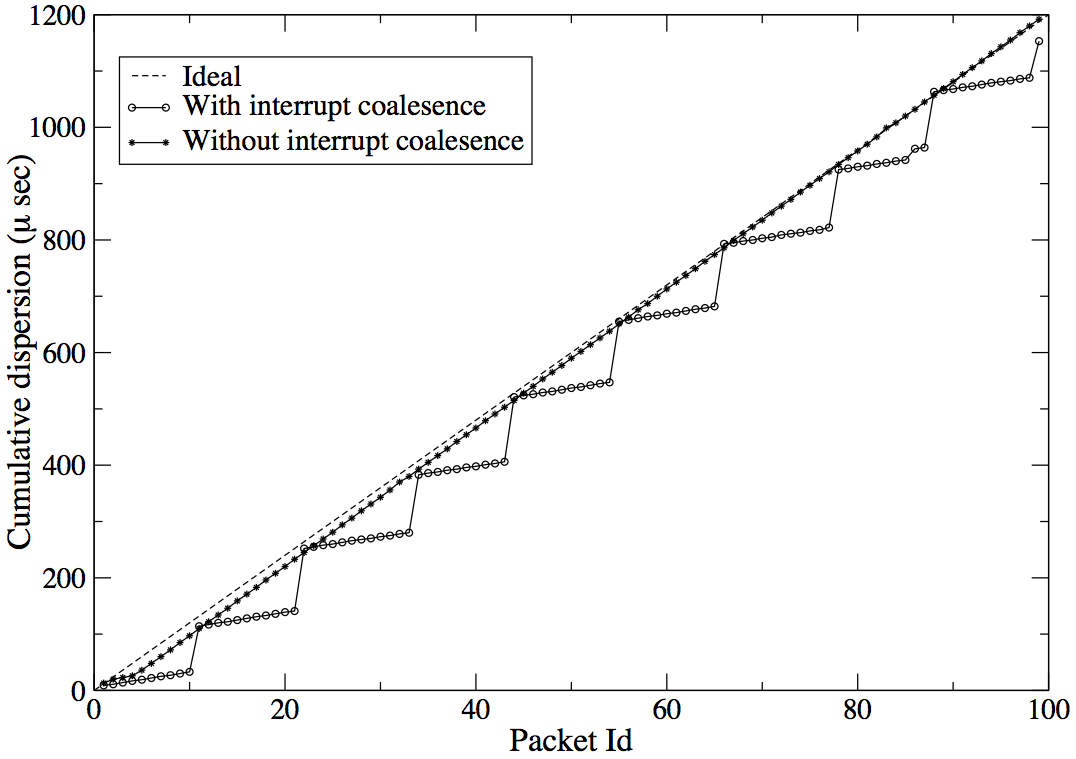
\includegraphics[width=0.8\textwidth]{interrupt-coalescence-wired}
  \end{figure}
}

\frame{\frametitle{Interrupt Coelescence (cont.)}
  On mobile devices, this mechanism is often adaptive, which means it is not so
  predictable from application's code.  Moreover:
  %
  \begin{itemize}
  \item implementation parameters may vary among different device drivers
  \item cross-traffic and contention of the physical medium can also alter the regularity of the pattern
  \end{itemize}
 }
 
 \frame{\frametitle{Interrupt Coelescence (cont.)}
 
   \begin{figure}
  \centering
  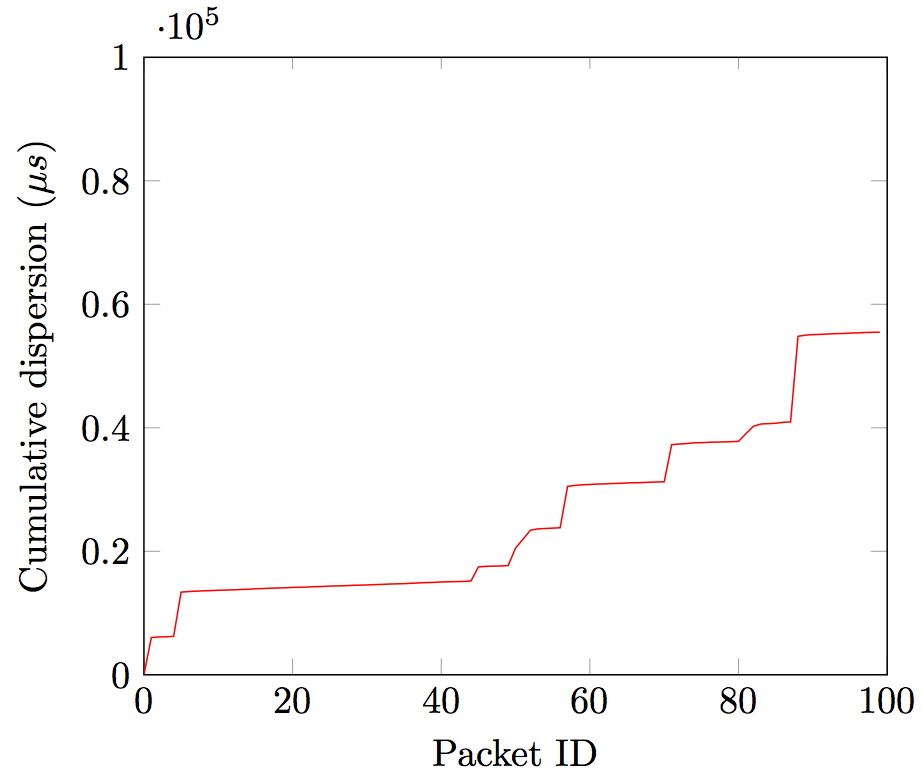
\includegraphics[width=0.7\textwidth]{interrupt-coalescence-wireless}
  \end{figure}
  
}

\frame{\frametitle{Interrupt Coelescence (cont.)}
  The presence of IC at the receiver's NIC can be detected by sending a long
  (but as small as possible) back-to-back packet train from the sender to the
  receiver and comparing measured dispersions with the kernel-to-user latency
  $\delta_\textup{k-u}$.
  
  \bigskip
  Problems:
  \begin{itemize}
  \item timer resolution can be smaller than $\delta_\textup{k-u}$
  \item kernel can adapt CPU frequency to computational load and battery level
  \item in the NIC's buffer there're packets for other applications
% TODO: in questo caso non comprimerei there're
  \item heights of jumps depend on many factors (length of IC's lapse, context switch, etc)
  \end{itemize}
 
  
  
}


\frame{\frametitle{Interrupt Coelescence (cont.)}
  Therefore, calculate capacities dividing each plateau's length for the 
  height of its jump can lead to errors of measurement.
    
  \begin{figure}
  \centering
  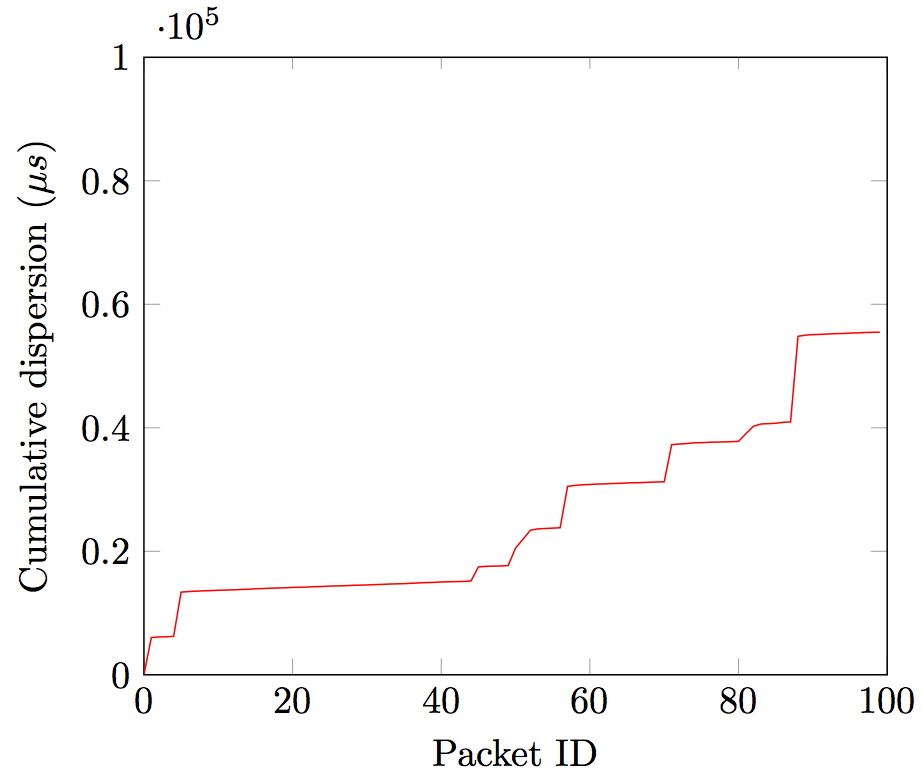
\includegraphics[width=0.5\textwidth]{capacity-plateau}
  \end{figure}


}




\section{SmartPathrate}
\frame{
  \sectionpage
}

\subsection{Objectives}

\frame{\frametitle{Our objectives}
  The execution of our application
  \begin{itemize}
  \item should not take a long time
    \begin{itemize}
    \item user wants to have a result quickly
    \item battery life should not be significantly affected
    \end{itemize}
  \item should not require too much resources
    \begin{itemize}
    \item processing complexity of mathematical computations
    \item memory usage for buffering partial results
    \end{itemize}
  \item should use as less data as possible
    \begin{itemize}
    \item mobile data plan may have traffic limitations
    \item more data means more processing
    \end{itemize}
  \end{itemize}
}

\subsection{The core procedure}

\frame{\frametitle{The core procedure}
  \begin{enumerate}
  \item Start with trains of 40 packets
  \begin{itemize}
  \item small trains are more likely to be successfully received
  \item it should be sufficient to avoid IC plateaus
  \end{itemize}
  \item Each round
  \begin{itemize}
  \item send 10 trains of the current length
  \item do calculations
  \item increment train length by 20\%
  \end{itemize}
  \item The longer the train, the more accurate the ADR estimation
    \begin{itemize}
    \item if cannot successfully receive trains, decrease train length by 5\%
    \item then, continue using the same length as far as no problem occurs
  % Treni lunghi: all'inizio l'interfaccia (o il kernel) può avere velocità
  % ridotta. È anche vero che il kernel può rispondere con la coalescenza.
  % La lunghezza dei treni deve esser tale da consentirci di avere almeno un
  % intervallo di coalescenza.
    \end{itemize}
  \end{enumerate}
}

\frame{\frametitle{The core procedure (cont.)}
  For every train in each round:
  \begin{itemize}
  \item Calculate capacities from successive packets in the train
    \begin{itemize}
    \item filter and remove dispersions affected by IC
    \end{itemize}
  \item Calculate ADR
    \begin{itemize}
    \item ignore if coalescence affects the beginning or the end of the train
    \end{itemize}
  \item Calculate bin width, distribution and modes of all gathered path and
        ADR capacities
  \item Try to determine the path capacity
  \end{itemize}
}

\subsection{Detect interrupt coalescence}

\frame{\frametitle{Detect Interrupt Coalescence}
  \begin{block}{Filtering capacities from IC}
  Detecting interrupt coalescence is a critical task
  \end{block}
  \pause

  \medskip
  \begin{exampleblock}{Idea}
  Why don't we reduce the receiver's buffer size by means of \texttt{setsockopt},
  to reduce or completely suppress IC?
  \end{exampleblock}
  \pause

  \medskip
  Option \texttt{SO\_RCVBUF} affects only a buffer related to the \emph{UDP
  socket}, and has nothing to do with the kernel's buffer used by NIC.

  In fact, the receiver's buffer should be as large as possible, to reduce
  (late) packet drops.
}

\frame{\frametitle{Detect Interrupt Coalescence}
  \begin{itemize}
  \item Is is accomplished by extracting two features from timestamps:
    \begin{enumerate}
    \item packet pair dispersions, compared to the \emph{kernel-to-user latency}
    \item variation of packet pair dispersion, compared to the \emph{minimum
          possible dispersion}
    \end{enumerate}
  \item Kernel-to-user latency is determined by sending and receiving packets
        via the loopback interface
    \begin{itemize}
    \item calculated just once after creating the UDP socket
          % We assume that CPU's frequency remain constant during the execution
          % of our application
    \end{itemize}
  \item Minimum possible delta is determined from the speed of local wireless
        link
    \begin{itemize}
    \item recalculated at each round, to adapt to changes in NIC's rate
    \end{itemize}
  \end{itemize}
}

\frame{\frametitle{}
  \begin{itemize}
  \item 
  \item Check for convergence of partial results
  \end{itemize}
}

\frame{
  Da un lato, misurare l'ADR, dall'altro le capacità dei plateau, in modo da
  avere una limite inferiore e un limite superiore ai valori di capacità
  accettabili.

  Possiamo cioè calcolare i valori di capacità propri dei plateau in modo da
  eliminare le relative mode dalla distribuzione di probabilità delle coppie di
  pacchetti.
  
  (Valutare se va bene calcolare le capacità tra le coppie anche se si è mandato
  un treno.)
}


\iffalse
@inproceedings{
  title = {Beyond Softnet},
  author = {Hadi Salim, Jamal and Olsson, Robert and Kuznetsov, Alexey},
  journal = {Proceedings of the 5th Annual Linux Showcase \& Conference},
  institution = {USENIX Association},
  year = 2001,
  location = {Oakland, California, USA},
  url = {http://static.usenix.org/publications/library/proceedings/als01/full_papers/jamal/jamal.pdf},
}

@book{linux-dev-drivers,
  title = {Linux Device Drivers},
  author = {Corbet, Jonathan and Rubini, Alessandro and Kroah-Hartman, Greg},
  publisher = {O'Reilly},
  edition = {Third edition},
  year = 2005,
  url = {http://lwn.net/images/pdf/LDD3/ch17.pdf},
}

@online{socket-buffers,
  notes = {%
    \url{http://unix.stackexchange.com/questions/74436/socket-buffer-and-purpose-of-so-rcvbuf},
    \url{http://datatag.web.cern.ch/datatag/papers/tr-datatag-2004-1.pdf},
    \url{http://www.6test.edu.cn/~lujx/linux_networking/0131777203_ch25lev1sec3.html},
    \url{http://vger.kernel.org/~davem/skb_sk.html},
    \url{http://www.haifux.org/lectures/217/netLec5.pdf}},
}
\fi

\end{document}
